% --------------------------------------------------------------------------------

\begin{exercise}

Programmieren Sie eine Gauss-Quadratur mit $m$ Stützstellen in einem Intervall $(a, b)$.
Verwenden Sie dazu die Berechnung der Stützstellen und Gewichte über das Eigenwertproblem der Tridiagonalmatrix

\begin{align}
  \begin{pmatrix}
    0       & \beta_1 &             &             & \\
    \beta_1 & 0       & \ddots      &             & \\
            & \ddots  & \ddots      & \beta_{n-2} & \\
            &         & \beta_{n-2} & 0           & \beta_{n-1} \\
            &         &             & \beta_{n-1} & 0
  \end{pmatrix}
  \in
  \R^{n \times n},
  \quad
  \beta_n = \frac{n}{\sqrt{4n^2 -1}}
\end{align}

Für letzeres können Sie einen fertigen Eigenwertlöser verwenden.
Testen Sie ihr Programm an unterschiedlichen Funktionen.
Bestimmen Sie dafür den Quadraturfehler numerisch und vergleichen Sie ihn mit theoretischen Fehlerschranken.

\end{exercise}

% --------------------------------------------------------------------------------

\begin{solution}

In unserem Fall ist die Gewichtsfunktion (vermutlich) $\omega \equiv 1$.

\includegraphicsboxed[Nannen - Numerik A]{Nannen - Numerik A - Satz 4.18.png}

Wir bekommen in unserem Fall also folgende (mehr oder weniger scharfe) Schranken.

\begin{align*}
  Q(f) - Q_n(f)
  \leq
  \frac
  {
    \norm[\infty]{f^{(2n+2)}}
  }{
    (2n + 2)!
  }
  (b - a)^{(2n+3)}
  =:
  \varepsilon_f(n)
\end{align*}

Zur Bestimmung der Knoten und Gewichte verwenden wir das Resultat aus Abbildung \ref{fig:NNAS4.23}.

\begin{figure}[h!]
  \begin{boxedin}
    \begin{center}
      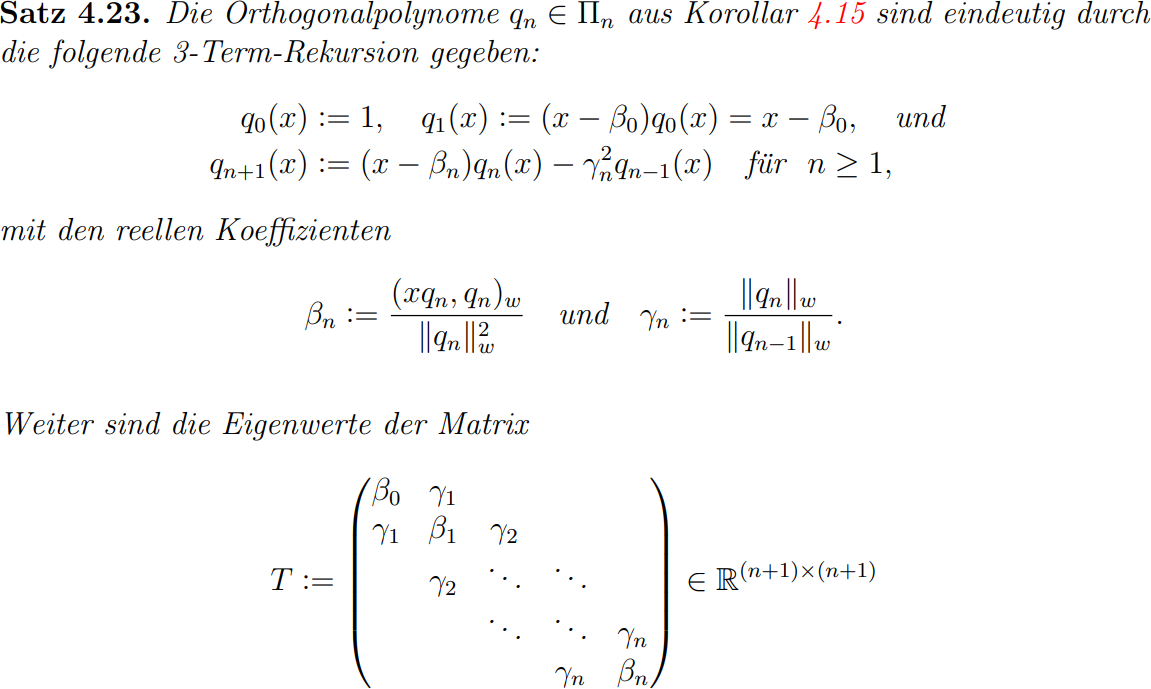
\includegraphics[width = 0.75 \textwidth]{Nannen - Numerik A - Satz 4.23.1.png} \\
      \vspace{0.5 cm}
      
\includegraphics[width = 0.75 \textwidth]{Nannen - Numerik A - Satz 4.23.2.png}
      \caption{Nannen - Numerik A}
      \label{fig:NNAS4.23}
    \end{center}
  \end{boxedin}
\end{figure}

Um von einem einem beliebigen Intervall $[a, b]$ auf das Referenz-Intervall $[-1, 1]$ zu transformieren, verwenden wir den Diffeomorphismus $\Phi^{-1}$.

\begin{align*}
  \Phi:
  [-1, 1] \to [a, b]:
  \xi \mapsto \Frac{2}{a + b + \xi (b - a)} \\
  \implies
  \Phi^{-1}:
  [a, b] \to [-1, 1]:
  \eta \mapsto \Frac{b-a}{2 \eta - (a + b)},
  \quad
  \Phi^\prime \equiv \frac{b - a}{2} \\
  \implies
  \Int[a][b]{f(x)}{x}
  \stackrel{\text{TRAFO}}{=}
  \frac{b - a}{2}
  \Int[-1][1]{f(\Phi(\xi))}{\xi}
\end{align*}

\end{solution}

% --------------------------------------------------------------------------------
